Quando parliamo di equilibrio chimico omogeneo, con \textit{omogeneo} intendiamo che tutti i composti presenti nella reazione (reagenti e prodotti) sono nella stessa fase, con \textit{equilibrio} intendiamo che a un certo punto si raggiunge una situazione in cui apparentemente non varia più la reazione. Tale situazione è detto di equilibrio.
\subsection{La costante di equilibrio}
Consideriamo la reazione tra idrogeno gassoso e iodio gassoso (cosa non naturale per lo iodio in quanto è un solido. Ciò significa che lo abbiamo riscaldato per portarlo in fase vapore):

$$\ce{H_2(g) + I_2(g) <--> 2HI(g)}$$
\vspace{-1cm}\begin{figure}[htp]
    \centering
    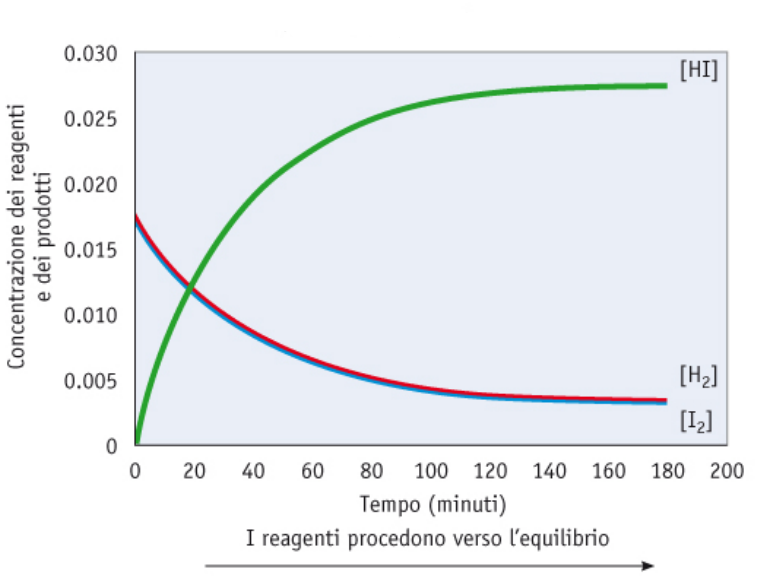
\includegraphics[width=10cm]{immagini/equilibrio_chimico.png}
\end{figure}

Il significato della doppia freccia è che la reazione può procedere in entrambi i sensi: sia da destra verso sinistra che da destra verso sinistra.

I due reagenti considerati danno luogo alla formazione di acido iodidrico, gassoso anch'esso.

L'equilibrio allora è omogeneo perché il prodotto ed entrambi i reagenti sono nella stessa fase.

Il grafico ci mostra che in questa particolare reazione le concentrazioni iniziali dei due reagenti sono uguali (non è necessario, ma conviene), mentre quella iniziale del prodotto è zero, cioè non c'è prodotto al tempo $t=0$.

Appena mescoliamo i reagenti e li facciamo reagire, immediatamente si forma acido iodidrico, ossia la reazione procede da sinistra verso destra.

Nell'istante in cui abbiamo già dell'acido iodidrico formato, piano piano parte la reazione opposta: l'acido si ridissocia per ridare nuovamente i reagenti.

Dato che ciò avviene subito, il processo sarà continuo.

Chiaramente alla fine ci sarà una parte dei reagenti che non ha reagito (o meglio, reagiscono ma poi si ridissociano). Le concentrazioni finali di H$_2$, I$_2$ e HI dipenderanno dalla concentrazioni iniziali di idrogeno e iodio.

\E importante che questa processo avvenga a temperatura fissata.

Si dimostra poi che il rapporto tra la concentrazione (indicata con le parentesi quadre) al quadrato del prodotto HI\footnote{eleviamo perché avevamo coefficiente stechiometrico pari a 2, cioè il coefficiente diventa espondente.} e il prodotto delle concentrazioni dei reagenti (ognuna elevata a 1 perché il loro coefficiente stechiometrico è 1) resta costante nel tempo, ossia è come se non cambiasse per le concentrazioni:

$$\rm \frac{[HI]^2}{[H_2] \cdot [I_2]}=cost$$

In questa fase diciamo che il sistema ha raggiunto l'equilibrio, cioè quando la reazione è in equilibrio tale rapporto non cambia più.

Inoltre possiamo anche partire da concentrazioni diverse tra loro dei reagenti. Ciò che cambierà sarà l'HI finale, ma quel rapporto rimane invariato, a patto che sia mantenuta fissa la temperatura.

Il valore di tale rapporto si chiama \textbf{costante di equilibrio}.

La reazione di ri-dissociazione ha una sua velocità, che è inizialmente diversa dalla reazione di partenza. Da un punto di vista cinetico possiamo dire che abbiamo raggiunto l'equilibrio quando la velocità di trasformazione dei reagenti in prodotto e quella dei prodotti in reagenti si eguagliano. A quel punto si dice che il sistema ha raggiunto l'equilibrio chimico, cioè alla fine le velocità saranno uguali.

Chiaramente anche questo è un equilibrio dinamico, non statico. Ciò significa che le concentrazioni sono fissate, non cambiano, ma ciononostante dell'idrogeno e dello iodio continueranno a reagire per formare dell'acido iodidrico e dell'acido iodidrico si dissocerà per ripristinare idrogeno e iodio in modo continuo. Quindi le reazioni non si fermano, ma non ce ne accorgiamo perché le quantità non cambiano, ossia da un punto di vista delle concentrazioni diciamo che queste sono ormai costanti.

Inoltre in questa reazione non cambia il numero di moli: due moli di reagenti danno due moli di prodotto. Si tratta di un caso particolare, in generale il numero di moli tra reagenti e prodotti varierà.

\vspace{0.2cm}Consideriamo adesso questa reazione:

$$\ce{2NO(g) + 2H_2(g) <--> 2H_2O(g) + N_2(g)}$$

In essa a due moli di ossido di azoto aggiungiamo due moli di idrogeno, per un totale di 4 moli. Tuttavia otteniamo due moli di acqua più una di azoto, per un totale di 3 moli.

Partiamo quindi da 4 moli di reagenti e otteniamo 3 moli di prodotti, dunque questa è una reazione in cui il numero di moli cambia. \E però anche questa una reazione di equilibrio, pertanto diremo che essa è in equilibrio quando sia temperatura e pressione fissate all'inzio, che le concentrazioni, sono costanti.

Una volta raggiunto l'equilibrio non si otterrà ulteriore reagente. Se però rompiamo l'equilibrio sottraendo un prodotto, la reazione cercherà di ripristinare ciò che ha sottratto, ovvero la reazione ripartirà producendo il reagente sottratto.

\vspace{0.2cm}Da un punto di vista cinetico, affinché due o più molecole reagiscano è necessario che

\begin{itemize}
    \item Le molecole si urtino, quindi non possiamo lavorare con sistemi assolutamente ideali in cui i gas sono rarefatti e si comportano come se fossero l'unico presente, perché in tali condizioni non ci sarebbero urti;
    \item L'urto sia efficace, ossia deve dare luogo ad atto reattivo. Per avvenire ciò le molecole devono possedere energia sufficiente per produrre i prodotti (atto reattivo). Ovviamente solo una percentuale delle molecole possiederà tale energia.

    Si osserva che più il sistema è concentrato, maggiore è la probabilità che ci siano molecole che si urtino.
\end{itemize}

Inoltre la velocità della reazione è proporzionale alla concentrazione, quindi all'inizio è massima la velocità verso destra, perché abbiamo massima concentrazione. Nell'istante in cui la reazioni parte, diminuisce la concentrazione dei reagenti e inizia a crescere quella dei prodotti, dunque col procedere della reazione la velocità verso destra diminuisce e aumenta la velocità verso sinistra. Quando queste due velocità sono uguali siamo all'equilibrio.
\subsection{La legge delle masse}
Cerchiamo di capire da dove venga l'idea di un quoziente di reazione in cui al numeratore ci sono le concentrazioni dei prodotti e al denominatore quelle dei reagenti, elevate ciascuna per il proprio coefficiente stechiometrico.

Va da notare che stiamo lavorando con speci in fase gassosa, quindi ancora prima delle concentrazioni conosciamo le pressioni parziali di queste speci, date dal valore delle tensioni di vapore proprie delle sostanze pure per la frazione molare. Ragioniamo quindi in termini di pressione parziale esercitata da ciascuna specie gassosa.

Consideriamo due reagenti A e B, che reagiscono (in una reazione di equilibrio) per produrre i prodotti C e D:

$$\ce{\alpha A + \beta B <--> \gamma C + \delta D}$$

dove $\alpha$, $\beta$, $\gamma$ e $\delta$ sono i coefficienti stechiometrici. A, B, C e D sono speci chimiche gassose del sistema in equilibrio.

Indichiamo poi con $G_A^0$, $G_B^0$, $G_C^0$ e $G_D^0$ le energie libere molari standard\footnote{L'energia libera di Gibbs (o entalpia libera) è una funzione di stato usata per rappresentare l'energia libera, cioè il lavoro che il sistema può compiere sull'ambiente.} (cioè a 25° C e e 1 atm) delle relative speci.

Indicheremo con $G_A$, $G_B$, $G_C$ e $G_D$ le energie libere molari a 25° C ma rispetto alle pressioni parziali finali di quando abbiamo raggiunto l'equilibrio.

Immaginiamo di avere eseguito una reazione e di essere passati da uno stato 1 a uno stato 2, in cui lo stato iniziale è a condizioni standard e lo stato finale è a condizioni di equilibrio, quindi ogni specie inizialmente aveva la pressione di 1 atm e alla fine avrà la pressione parziale $P_A$, $P_B$, $P_C$ o $P_D$. La variazione di energia libera in questa reazione sarà data Da

$$\Delta G = RT \ln \frac{P_2}{P_1}, \quad \Delta G = G - G^0$$

La variazione di energia libera per ogni specie sarà

$$\Delta G_A = \alpha G_A - \alpha G_A^0 = \alpha RT \ln \frac{P_A}{1}$$

Tuttavia la variazione di energia libera all'equilibrio (cioè quando una reazione ha raggiunto l'equilibrio) è pari a zero. Segue che

$$\alpha G_A = 0 \implies \alpha G_A = \alpha G_A^0  + \alpha RT \ln P_A$$

Analogamente

$$\beta G_B = \beta G_B^0  + \beta RT \ln P_B,
\quad
\gamma G_C = \gamma G_C^0  + \gamma RT \ln P_C,
\quad
\delta G_D = \delta G_D^0  + \delta RT \ln P_D$$

Possiamo allora calcolare un $\Delta G$ della reazione, dato dalla variazione di energia libera dei prodotti meno la variazione di energia libera dei reagenti.

$$\Delta G_{reazione} = (\gamma G_C + \delta G_D) - (\alpha G_A + \beta G_B)$$

sostituendo

$$\Delta G = (\gamma G_C^0  + \gamma RT \ln P_C + \delta G_D^0  + \delta RT \ln P_D) - 
(\alpha G_A^0  + \alpha RT \ln P_A + \beta G_B^0  + \beta RT \ln P_B)$$

$$\implies \Delta G = \gamma G_C^0 + \delta G_D^0 - \alpha G_A^0 - \beta G_B^0 + RT \ln \frac{P_C^{\gamma} \cdot P_D^{\delta}}{P_A^{\alpha} \cdot P_B^{\beta}}$$

Va da notare che l'argomento del logaritmo è il prodotto delle pressioni dei prodotti, diviso il prodotto delle pressioni parziali dei reagenti, dove ciascuna di queste pressioni è elevata per il proprio coefficiente stechiometrico.

All'equilibrio $\Delta G = 0$. Inoltre Poniamo

$$\Delta G^0 = \gamma G_C^0 + \delta G_D^0 - \alpha G_A^0 - \beta G_B^0 $$

Segue che

$$\Delta G^0 = -RT \ln \frac{P_C^{\gamma} \cdot P_D^{\delta}}{P_A^{\alpha} \cdot P_B^{\beta}}$$

A T costante $\Delta G^0$ è un numero. Ne segue che anche l'argomento del logaritmo sarà uguale a una costante, la quale è funzione delle pressioni parziali. Tale costante è detta \textit{costante di reazione} $k_p$. L'espressione allora diventa

$$\frac{P_C^{\gamma} \cdot P_D^{\delta}}{P_A^{\alpha} \cdot P_B^{\beta}} = k_p
\implies
\Delta G^0 = -RT\ln k_p$$

Se la costante $k_p$ viene espressa in funzione delle concentrazioni diventa il rapporto delle concentrazioni visto all'inizio e che non cambia nonostante le concentrazioni iniziali.

QUindi, qualunque siano le condizioni iniziali, purché sia fissata la temperatura, il valore della costante $k_p$ non cambia per ogni reazioni, cioè ogni reazione ha la sua costante che non cambia se non cambia la temperatura, ma che non cambia anche se cambiano le concentrazioni di reagenti e di prodotti.

Va da notare che le pressioni parziali che figurano in essa sono quelle all'equilibrio e non quelle iniziali.

Analogamente se la esprimiamo con le concentrazioni.
\subsection{Relazione tra $k_p$ e $k_c$}
Sriamo parlando di equilibri in fase gassosa e quindi di reazioni in fase gassosa, nonché di pressioni parziali di ciascuno dei componenti. Noi però siamo abituati a lavorare in soluzione, pertanto laddove fosse possibile vogliamo capire come fare per ragionare su equilibri in soluzione acquosa (per possibile si intende avere speci che si sciolgono in acqua). Quello che vogliamo quindi capire è se c'è una relazione tra la costante di equilibrio in funzione delle pressioni parziali $k_p$ e la costante di equilibrio in funzione della concentrazione $k_c$.

La $k_p$ della reazione è

$$k_p = \frac{P_C^{\gamma} \cdot P_D^{\delta}}{P_A^{\alpha} \cdot P_B^{\beta}}$$

Dall'equazione di stato dei gas si ha

$$PV=nRT \implies P=\frac{n}{V}RT \implies P=c \cdot RT$$

Se indichiamo con [A], [B], [C] e [D] le varie concentrazioni, la $k_p$ sarà

$$k_p = \frac{[\text{C}]^{\gamma} [\text{D}]^{\delta}}{[\text{A}]^{\alpha} [\text{B}]^{\beta}} \cdot \frac{(RT)^{\gamma} (RT)^{\delta}}{(RT)^{\alpha} (RT)^{\beta}}$$

Poniamo

$$k_c = \frac{[\text{C}]^{\gamma} [\text{D}]^{\delta}}{[\text{A}]^{\alpha} [\text{B}]^{\beta}}, \quad \Delta n= (\gamma + \delta - \alpha - \beta)$$

Scriveremo che

$$k_p = k_c \cdot (RT)^{\Delta n}$$

$\Delta n$ è la variazione del numero di moli. Se le moli di reagenti sono uguali in numero a quelle dei prodotti $\Delta n$ sarà pari a zero, per cui $k_p = k_c$. In caso contrario, cioè se cè variazione del numero di moli, $\Delta n \neq 0$ e $k_p \neq k_c$

\vspace{0.2cm}\textbf{Es.1}
$$\ce{H_2 + I_2 <--> 2HI}, \quad \Delta n = 0 \implies k_p = k_c$$

\textbf{Es.2}
$$\ce{PCl_5  <--> PCl_3 + Cl_2}, \quad \Delta n = 1 \implies k_p = k_c - RT$$
\subsection{Fattori che influenzano l'equilibrio}

\subsubsection{Influenza della pressione}
Ragioniamo adesso su cosa succede se modifichiamo la pressione, cioè vogliamo capire se la costante di equilibrio dipende anche dalla pressione.

La pressione di ciascun componente è data dalla pressione totale per la sua frazione molare, ad esempio la pressione del componente A sarà $P_A = P_{tot} \cdot \rchi_A$.

Se allora abbiamo una reazione del tipo

$$\ce{\alpha A + \beta B <--> \gamma C + \delta D}$$

la costante di equilibrio potrà essere scritta come

$$k_p = \frac{P_C^{\gamma} \cdot P_D^{\delta}}{P_A^{\alpha} \cdot P_B^{\beta}} = \frac{\rchi_C^{\gamma} \cdot \rchi_D^{\delta}}{\rchi_A^{\alpha} \cdot \rchi_B^{\beta}} \cdot P_{tot}^{(\gamma + \delta - \alpha - \beta)}$$

$$\implies k_p = k_{\rchi} \cdot P^{\Delta n}$$

cioè la $k_p$ è uguale alla costante espressa in funzione delle frazioni molari per la pressione totale elevata alla variazione del numero di moli:

\begin{itemize}
    \item Se $\Delta n = 0 \implies k_p = k_{\rchi}$
    \item Se $\Delta n \neq 0 \implies k_p \neq k_{\rchi}$
\end{itemize}

\vspace{0.2cm}\textbf{Es.1}
$$\ce{H_2 + I_2 <--> 2HI}, \quad \Delta n = 0 \implies k_p = k_{\rchi}$$

\textbf{Es.2}
$$\ce{2NO + O_2 <--> 2NO_2}, \quad \Delta n = -1 \implies k_p = k_{\rchi} \cdot P^{-1}$$

$$\implies k_p = k_{\rchi} \cdot \frac{1}{P}= \frac{\rchi_{NO_2}^2}{\rchi_{NO}^2 \cdot \rchi_{O_2}} \cdot \frac{1}{P}$$

Dall'ES.2 deduciamo che $k_p$ è inversamente proporzionale alla pressione totale.

Se aumenta la pressione, affinché il rapporto resti costante dovrà aumentare il numeratore. Nel caso particolare dovrà allora aumentare la frazione molare di $NO_2$.

Ne segue che so vogliamo spostare l'equilibrio verso destra, il che equivale a produrre più $NO_2$ di quanto ne produce già la reazione, dobbiamo comprimere. Ciò faciliterà anche la diminuizione di volume (infatti da 3 moli di reagenti passiamo a 2 moli di prodotto) in questa specifica reazione.

\vspace{0.2cm}\textbf{Es.3 La produzione dell'ammoniaca}
$$\ce{N_2 + 3H_2 <--> 2NH_3}$$

In essa abbiamo 4 moli di reagente e due di prodotto.

La costante di equilibrio sarà

$$k_p = \frac{P_{NH_3}^2}{P_{N_2} + P_{H_2}^3}$$

In termini di frazione molare sarà

$$k_P = \frac{\rchi_{NH_3}^2}{\rchi_{N_2} + \rchi_{H_2}^3} \cdot \frac{1}{P^2}$$

Questa reazione allora sarà ancora di più influenzata dalla pressione.

\vspace{0.2cm}Quindi in una reazione non possiamo agire sulla temperatura perché cambierebbe la costante, ma fissata la temperatura possiamo variare l'equilibrio (cioè spostarlo più a destra o più a sinistra) cambiando il valore della pressione in tutte quelle reazioni laddove il numero di moli cambia con la reazione ($\Delta n \neq 0$).

\vspace{0.2cm}Va da notare che per $\Delta n > 0$, cioè se il numero di moli nei prodotti aumenta, per spostare l'equilibrio verso destra si deve abbassare la pressione.

\subsubsection{Influenza della temperatura}
Abbiamo detto che la temperature non puà variare, altrimenti cambia il valore della costante di equilibrio.

Consideriamo la reazione

$$\ce{N_2(g) + O_2(g) + 180.5 \, kJ/mol <--> 2NO(g)}$$

Per ottenere l'ossido di azoto dobbiamo riscaldare, cioè dobbiamo fornire calore. Abbiamo quindi immaginato che il calore sia un reagente.

Siccome questo processo richiede assorbimento di calore, cioè il processo è endotermico e $\Delta$H$>0$. Aumentare calore comporterà allora un aumento del prodotto ottenuto, perché è come se aumentassimo la concentrazione dei reagenti. Il calore quindi è diventato un reagente, tant'è che la costante di equilibrio aumenta con la temperatura.

Pertanto se il calore è un reagente, l'equilibrio può essere spostato verso destra fornendo calore.

Consideriamo adesso la reazione

$$\ce{2NO_2(g) <--> N_2O_4(g) + 57.2 \, kJ/mol}$$

Il biossido di azoto ha un elettrone spaiato sull'azoto, ossia è una molecola paramagnetica. Due molecole di NO$_2$ tendono a unire questi due elettroni spaiati e formare un legame, ottenendo così il dimero (cioè una molecola formata dall'unione di due molecole uguali) N$_2$O$_4$.

In questa reazione il calore è a destra, ossia questa reazione avviene con sviluppo di calore (processo esotermico, $\Delta$H$<$0. Allora per spostare l'equilibrio verso destra dovremo raffreddare, cioè sottrarremo il calore. Infatti la costante di equilibrio di questa reazione diminuisce all'aumentare della temperatura.

Quindi se la reazione sviluppa calore, sottraiamo questo e la reazione riparte per riprodurre il calore sottratto. In altre parole tutte le volte che c'è una reazione all'equilibrio e l'equilibrio viene turbato, esso si sposta da solo per tentare di ripristinare un nuovo stato di equilibrio.

Se invece la reazione necessita riscaldamento, riscaldando la reazione ripartirà.

In questo modo sarà come aumentare, rispettivamente, le concentrazioni dei prodotti e dei reagenti.

Sostanzialmente

\begin{itemize}
    \item L'aumento di T provoca l'aumento di $k_c$ se $\Delta$H$>$0 (endotermico)
    \item L'aumento di T provoca la diminuizione di $k_c$ se $\Delta$H$<$0 (esotermico)
\end{itemize}

Torniamo all'ultima reazione:

\begin{figure}[htp]
    \centering
    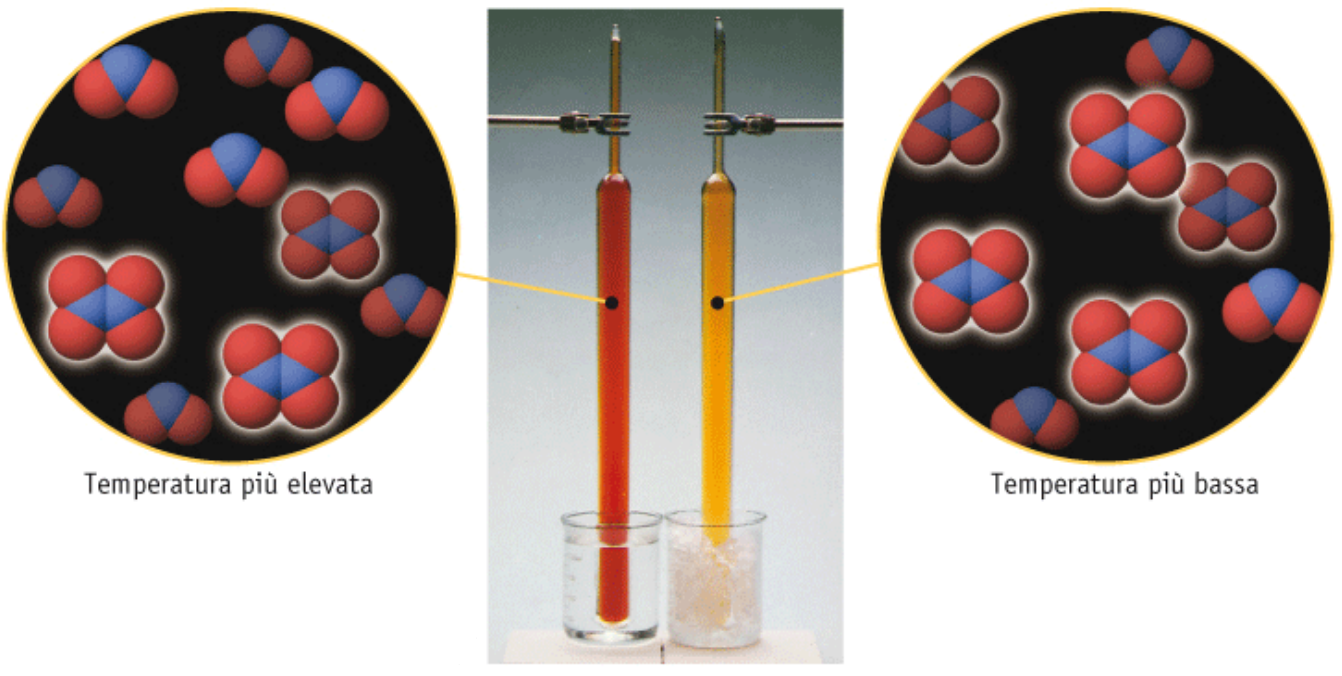
\includegraphics[width=10cm]{immagini/reazione_NO_2.png}
\end{figure}

NO$_2$ è una molecola paramagnetica perché ha un elettrone spaiato, mentre la molecola N$_2$O$_4$ non lo ha, quindi non è paramagnetica. L'elettrone spaiato fornisce un colore bruno all'NO$_2$, mentre N$_2$O$_4$ è incolore.

Nell'immagine sono mostrati due tubi, i quali contengono entrambi NO$_2$ e N$_2$O$_4$ all'equilibrio. Entrambi sono inoltre immersi in un recipiente, solo che quello che a sinistra contiene acqua a 50° C, quello a destra ghiaccio.

$k_c$ è più grande a temperatura più bassa, poiché l'equilibrio favorisce la produzione di N$_2$O$_4$ incolore. Ciò si osserva chiaramente nel tubo di destra, dove il contenuto è solo leggermente colorato, fatto che indica una bassa concentrazione del gas NO$_2$. A destra invece, dove la temperatura è maggiore, l'equilibrio è spostato verso NO$_2$, come è indicato dall'intensa colorazione marrone.

\vspace{0.2cm}Va poi da notare che se siamo in una reazione di equilibrio non scompariranno mai i reagenti, perché se scomparissero per dare solo prodotti non sarebbe più un equilibrio:

\begin{figure}[htp]
    \centering
    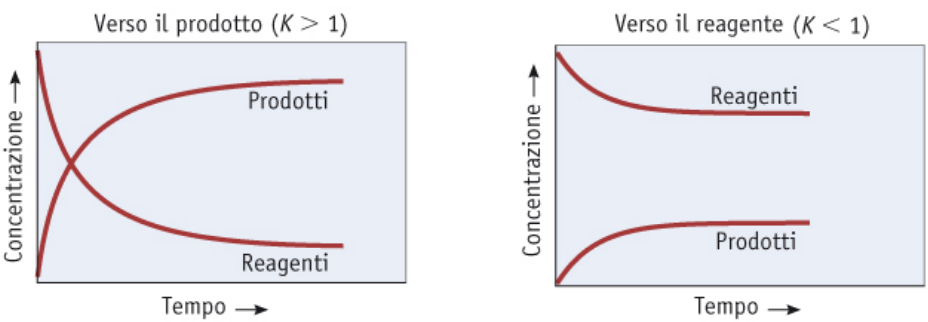
\includegraphics[width=16cm]{immagini/reazioni_equilibrio_spostato.png}
\end{figure}

Nel prima grafico abbiamo una certa concentrazione iniziale di reagenti che diminuisce fino a diventare costante quando viene raggiunto l'equilibrio mentre i prodotti inizialmente non esistevano, ma poi iniziano a formarsi fino a raggiungere una concentrazione costante all'equilibrio. Notiamo che la concentrazione finale dei reagenti è bassa, quella dei prodotti è alta. Possiamo allora dire che questa reazione è spostata verso destra, ossia verso i prodotti. Allora, per come è definita $k_c$, questa sarà maggiore di 1.

Se invece, come nel caso del secondo grafico, la concentrazione dei reagenti diminuisce ma resta lo stesso alta e i prodotti si formano poco cioè hanno una bassa concentrazione, all'equilibrio i reagenti saranno più presenti dei prodotti. Allora, sempre per la definizione di $k_c$, essa sarà minore di 1, ovvero la reazione è spostata verso sinistra, cioè forma poco prodotto: i reagenti restano largamente non reagiti.

\vspace{0.2cm}Quindi il valore di $k_c$ è indicativo di quanto la reazione procede verso destra.

Ad esempio il solfato di bario BaSO$_4$ ha una costante pari a $1.08 \cdot 10^{-10}$, cioè non si scioglie quasi per niente. Ecco perché si può bere.

Quindi l'equilibrio chimico può essere modificato cambiando le concentrazioni, la temperatura o la pressione:
\vspace{0.2cm}\begin{center}
\scriptsize\begin{tabular}{|l|l|l|l|}
    \hline
    & \textbf{Cambiamento quando la} &  &\\
    \textbf{Perturbazione} & \textbf{miscela torna all'equilibrio} & \textbf{Effetto sull'equilibrio} & \textbf{Effetto su $k$}\\
    \hline
    \textit{Reazioni coinvolgenti solidi,}&&&\\
    \textit{liquidi o gas} &&&\\[0.5ex]
    \hline
    Aumento della temperatura & Energia termica è consumata & Spostamento nella dire- & Cambiamento\\
    & dal sistema & zione endotermica &\\[0.5ex]
    \hline
    Diminuzione della & Energia termica è generata & Spostamento nella dire- & Cambiamento\\
    temperatura & dal sistema & zione esotermica &\\
    \hline
    Addizione di un reagente & Il reagente addizionato viene & Aumenta la concen- & Nessun\\
    & in parte consumato & trazione dei prodotti & cambiamento\\[0.5ex]
    \hline
    Addizione di un prodotto & Il prodotto addizionato viene & Aumenta la concen- & Nessun\\
    & in parte consumato & trazione dei reagenti & cambiamento\\[0.5ex]
    \hline
    \textit{Reazioni coinvolgenti gas} &&&\\[0.5ex]
    \hline
    Diminuzione del volume, & Diminuzione della pressione & La composizione cambia & Nessun\\
    diminuzione della pressione & & per ridurre il numero &cambiamento\\
    &&totale delle molecole&\\
    &&gassose&\\[0.5ex]
    \hline
    Aumento del volume, & Aumento della pressione & La composizione cambia & Nessun\\
    diminuzione della pressione & & per ridurre il numero &cambiamento\\
    &&totale delle molecole&\\
    &&gassose&\\
    \hline
\end{tabular}
\end{center}

\vspace{0.2cm}\normalsize La definizione della costante di equilibrio si ottiene però fissando la temperatura. La pressione invece non fa variare il valore della costante, ma ci permette, qualora avessimo variazione del numero di moli, di modificare le concentrazioni finali all'equilibrio.

La temperatura quindi modifica l'equilibrio. Tuttavia può essere necessario cambiarla qualora avessimo una reazione che sia un processo endotermico o esotermico. Se è un processo endotermico, che assrobe calore, riscaldare significherà favorirlo e quindi ottenere più prodotto; se è un processo esotermico, che sviluppa calore, per ottenere più prodotto conviene sottrarre calore.
\subsection{Produzione dell'ammoniaca}
Il progresso industriale di una nazione si misura in rapporto al numero di tonnellate di acido solforico e ammoniaca che produce in un anno.

In particolare l'ammoniaca viene prodotto attraverso il \textbf{processo di Haber-Bosch}.

\vspace{-1cm}\begin{figure}[htp]
    \centering
    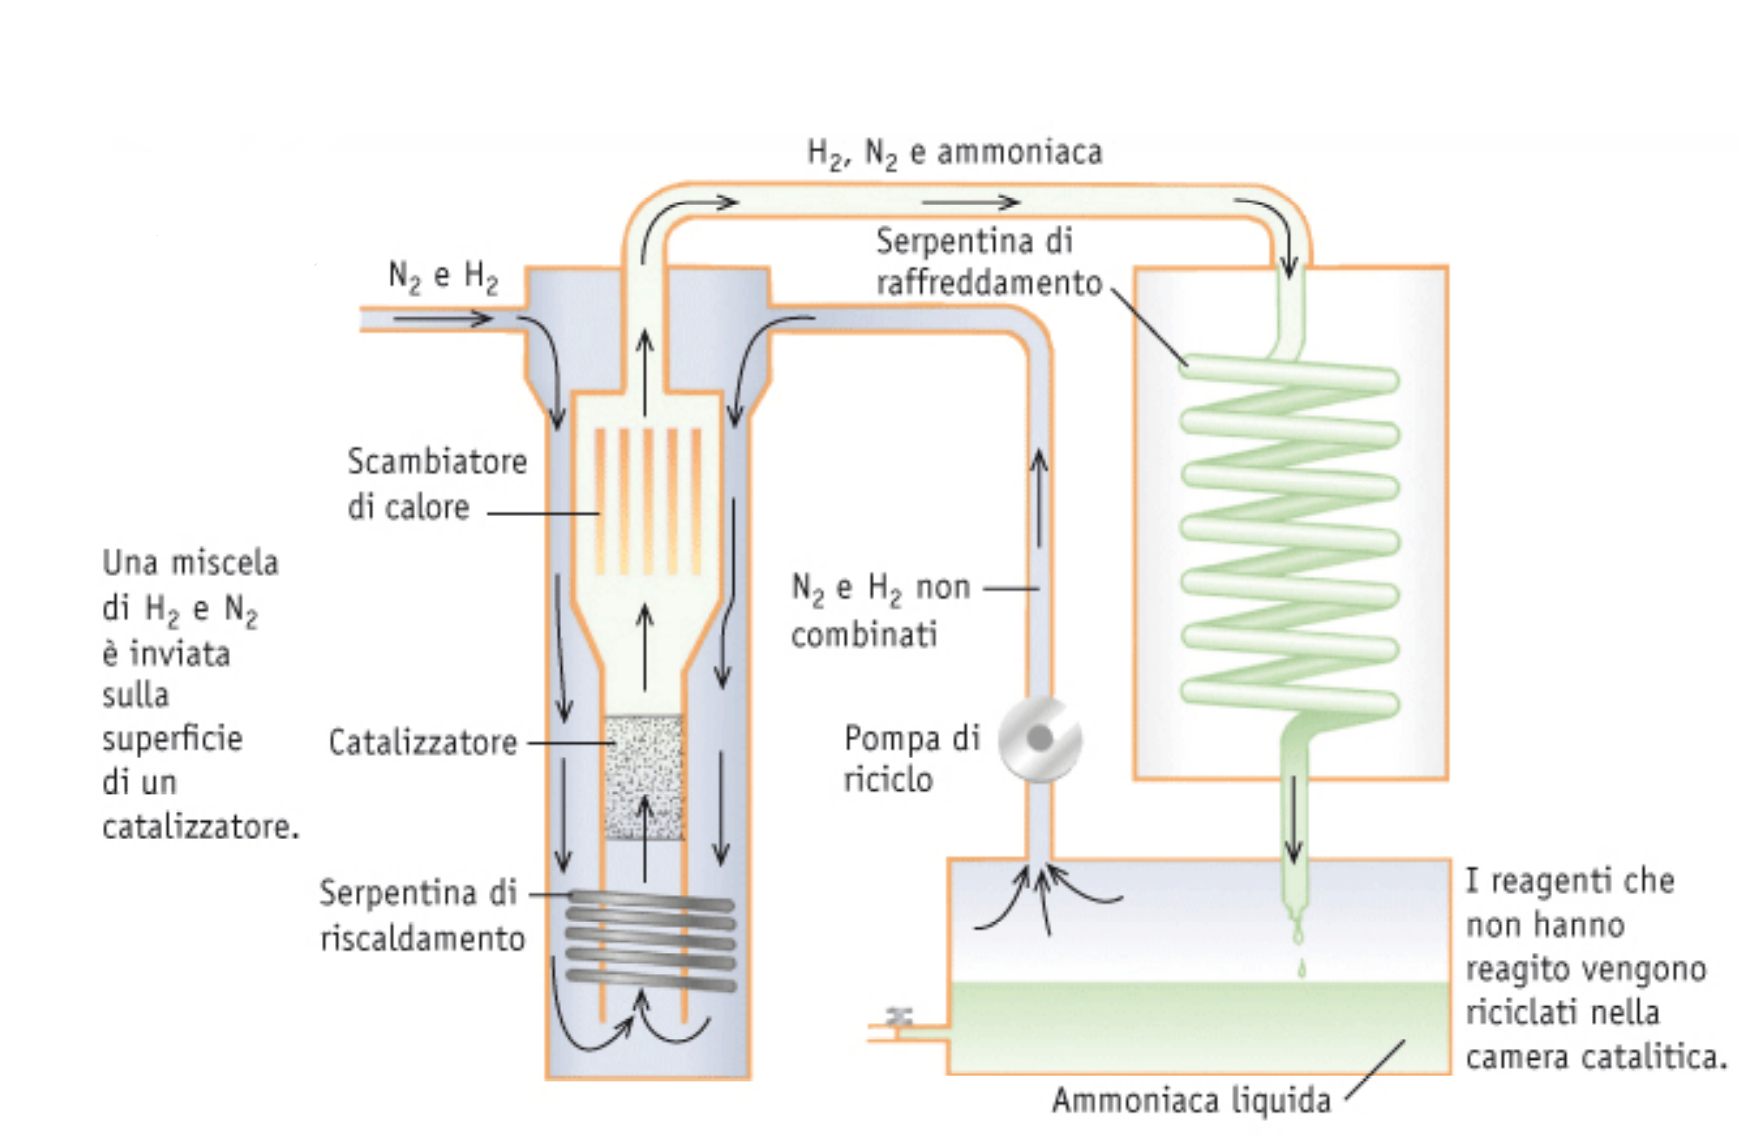
\includegraphics[width=14cm]{immagini/produzione_ammoniaca.png}
\end{figure}

In esso si parte da idrogeno ed azoto gassosi:

$$\ce{N_2(g) + 3H_2(g) <--> 2NH_3(g)}$$

Per avvenire da sola tale reazione, necessita temperature di circa 100=° C. Nella pratica però è possibile abbassare la temperatura a circa 400° C introducendo azoto e idrogeno in un sistema dotato di una serpentina che li riscalda e vengono fatti passare attraverso un catalizzatore che è l'F$_3$O$_4$, il quale, come si dice in gergo tecnico, permette di abbassare l'energia di attivazione della reazione. Si ottiene così dell'ammoniaca che va condensata a -33° C.

Tuttavia questa è una reazione di equilibrio, quindi parte dei reagenti resteranno non reagiti. Ci sarà allora una pompa che riaspira i gas non reagiti per rinviarli nel sistema e far ripartire il processo.
\newpage
\subsubsection{Valori vari della costante di equilibrio}

Riportiamo adesso alcuni esempi dei valori delle costanti di equilibrio.

\vspace{0.5cm}\hspace{-0.5cm}\scriptsize\begin{tabular}{p{3.4cm}p{1.6cm}p{2.5cm}p{3.4cm}p{1.6cm}p{2.5cm}}
    \textbf{Composto} & \textbf{Formula} & $\boldsymbol{K_{ps}}$ & \textbf{Composto} & \textbf{Formula} & $\boldsymbol{K_{ps}}$\\[0.7ex]
    Perclorato di potassio & KClO$_4$ & $1.05 \cdot 10^{-2}$ & Bromuro di magnesio & AgBr & $7.7 \cdot 10^{-13}$\\[0.7ex]
    Fluoruro di litio & LiF & $1.84 \cdot 10^{-2}$ & Idrossido di zinco & Zn(OH)$_2$ & $1.8 \cdot 10^{-14}$ (a 20° C)\\[0.7ex]
    Carbonato di litio & Li$_2$CO$_3$ & $1.7 \cdot 10^{-3}$ & Carbonato di piombo & PbCO$_3$ & $3.3 \cdot 10^{-14}$ (a 18° C)\\[0.7ex]
    Nitrato di argento & AgNO$_3$ & $5.86 \cdot 10^{-4}$ & Idrossido di manganese & Mn(OH)$_2$ & $4 \cdot 10^{-14}$ (a 18° C)\\[0.7ex]
    Bromato di bario & Ba(BrO$_3$)$_2$ & $2.43 \cdot 10^{-4}$ & Idrossido ferroso & Fe(OH)$_2$ & $1 \cdot 10^{-15}$ \\[0.7ex]
    Solfato di calcio & CaSO$_4$ & $4.93 \cdot 10^{-5}$ & Clpruro di Mercurio & HgCl$_2$ & $2.6 \cdot 10^{-15}$\\[0.7ex]
    Carbonato di magnesio & MgCO$_3$ & $2.6 \cdot 10^{-5}$ (a 12° C) & Idrossido di piombo & Pb(OH)$_2$ & $1 \cdot 10^{-16}$\\[0.7ex]
    Cloruro di piombo & PbCl$_2$ & $1.7 \cdot 10^{-5}$ & Ioduro di argento & AgI & $1.5 \cdot 10^{-16}$\\[0.7ex]
    Solfato di argneto & Ag$_2$SO$_4$ & $1.2 \cdot 10^{-5}$ & Idrossido di cromo (II) & Cr(OH)$_2$ & $2 \cdot 10^{-16}$ \\[0.7ex]
    Idrossido di calcio & Ca(OH)$_2$ & $5.02 \cdot 10^{-6}$ & Idrossido di nichel & Ni(OH)$_2$ & $5.48 \cdot 10^{-16}$ \\[0.7ex]
    Bicromato di argento & Ag$_2$Cr$_2$O$_7$ & $2 \cdot 10^{-7}$ & Solfuro ferroso & FeS & $3.7 \cdot 10^{-19}$ (a 18° C)\\[0.7ex]
    Iodato di rame & Cu(IO$_3$)$_2$ & $1.4 \cdot 10^{-7}$ & Idrossido di rame (II) & $\rm Cu(OH)_2$ & $4.8 \cdot 1o^{-20}$\\[0.7ex]
    Carbonato di calcio & CaCO$_3$ & $0.87 \cdot 10^{-8}$ & Bromuro di mercurio & HgBr$_2$ & $8 \cdot 10^{-20}$\\[0.7ex]
    Solfato di piombo & PbSO$_4$ & $1.06 \cdot 10^{-8}$ (a 18° C) & Fosfato di alluminio & AlPO$_4$ & $9.84 \cdot 10^{-21}$\\[0.7ex]
    Ioduro di piombo & PbI$_2$ & $1.39 \cdot 10^{-8}$ & Solfuro di manganese & MnS & $10^{-22}$\\[0.7ex]
    Idrossido di argento & AgOH & $1.52 \cdot 10^{-8}$ (a 20° C)& Idrossido di berillio & Be(OH)$_2$ & $6.92 \cdot 10^{-22}$\\[0.7ex]
    Fluoruro di piombo & PbF$_2$ & $3.2 \cdot 10^{-8}$ & Solfuro di zinco & ZnS & $1.2 \cdot 10^{-23}$ (a 18° C)\\[0.7ex]
    Fluoruro di magnesio & MgF$_2$ & $6.4 \cdot 10^{-9}$ & Idrossido stannoso & Sn(OH)$_2$ & $5.45 \cdot 10^{-27}$\\[0.7ex]
    Carbonato di bario & BaCO$_3$ & $8.1 \cdot 10^{-9}$ &Solfuro di stagno (II)  & SnS & $1 \cdot 10^{-28}$\\[0.7ex]
    Carbonato rameico & CuCO$_3$ & $1 \cdot 10^{-10}$ & Solfuro di piombo & PbS & $3.4 \cdot 10^{-28}$ (a 18° C)\\[0.7ex]
    Solfato di bario & BaSO$_4$ & $1.08 \cdot 10^{-10}$ & Ioduro di mercurio & HgI$_2$ & $3.2 \cdot 10^{-29}$ \\[0.7ex]
    Cloruro di argento & AgCl & $1.56 \cdot 10^{-10}$ & Idrossido di cromo (III) & Cr(OH)$_3$ & $6.3 \cdot 10^{-31}$\\[0.7ex]
    Idrossido di magnesio & Mg(OH)$_2$ & $1.2 \cdot 10^{-11}$ (a 18° C) & Idrossido di alluminio & Al(OH)$_3$ & $3 \cdot 10^{-34}$\\[0.7ex]
    Fluoruro di calcio & CaF$_2$ & $3.95 \cdot 10^{-11}$ & Solfuro rameoso & Cu$_2$S & $2 \cdot 10^{-47}$ (a 18° C)\\[0.7ex]
    Carbonato di manganese & MnCO$_3$ & $9 \cdot 10^{-11}$ & Solfuro di argento & Ag$_2$S & $1.6 \cdot 10^{-49}$ (a 18° C)\\[0.7ex]
    Carbonato di argento & Ag$_2$CO$_3$ & $6.15 \cdot 10^{-12}$ & Solfuro di mercurio & HgS & $1 \cdot 10^{-50}$ (a 18° C)\\[0.7ex]

\end{tabular}

\vspace{0.4cm}

\footnotesize\begin{tabular}{p{9.5cm}p{2.3cm}p{3.3cm}}
    & Costante di & Reazione spostata\\
    & equilibrio, $k$ & verso i prodotti o i\\
        Reazione & (a 25° C) & reagenti all'equilibrio\\
        \hline
        Reazione di combinazione di non metalli&&\\[0.5ex]
        \ce{S(s) + O_2(g) <--> SO_2(g)} & $4.2 \cdot 10^{52}$ & $k>1$; prodotti\\[0.7ex]
        \ce{2H_2(g) + O_2(g) <--> 2H_2O(g)} & $3.2 \cdot 10^{81}$ & $k>1$; prodotti\\[0.7ex]
        \ce{N_2(g) + 3H_2(g) <--> 2NH_3(g)} & $3.5 \cdot 10^8$ & $k>1$; prodotti\\[0.7ex]
        Reazioni di ionizzazione di acidi e basi deboli &&\\[0.5ex]
        \ce{HCO_2H(aq) + H_2O($l$) <--> HCO_2^-(aq) + H_3O^+} & $1.8 \cdot 10^{-4}$ & $k<1$; reagenti\\
        acido formico &&\\[0.7ex]
        \ce{CH_3CO_2(aq) + H_2O($l$) <--> CH_3CO_2^-(aq) + H_3O^+(aq)} & $1.8 \cdot 10^{-5}$ & $k<1$; reagenti\\
        acido acetico&&\\[0.7ex]
        \ce{H_2CO_3(aq) + H_2O($l$) <--> HCO_3^-(aq) + H_3O^+(aq)} & $4.2 \cdot 10^{-7}$ & $k<1$; reagenti\\
        acido carbonico&&\\[0.7ex]
        \ce{NH_3(aq) + H_2O($l$)} & $1.8 \cdot 10^{-5}$ & $k<1$; reagenti\\
        ammoniaca&&\\[0.7ex]
        Reazione di dissoluzione di solidi "insolubili"&&\\[0.7ex]
        \ce{CaCO_3(s) <--> Ca^{2+}(aq) + CO_3^{2-}(aq)} & $3.8 \cdot 10^{-9}$ & $k<1$; reagenti\\[0.7ex]
        \ce{AgCl(s) <--> Ag^+(aq) + Cl^-(aq)} & $1.8 \cdot 10^{-10}$ & $k<1$; reagenti\\[0.7ex]
\end{tabular}